\begin{sidewaysfigure}[!htp]
  \begin{minipage}{\linewidth}
    \caption{Interest Rate Differentials, Capital Intensity, and
      Exchange Rate Regimes \label{fig_stylized}}
    \label{fig_intro}
    \begin{subfigure}{.33\textwidth}
      \centering
      \caption{Interest Rate Differential (Resid.)}
      \includegraphics[width=\textwidth]{./Figures/Figure_FP_ERA.pdf}
    \end{subfigure}
    \begin{subfigure}{.33\textwidth}
      \centering
      \caption{Currency Excess Returns (Resid.)}
      \includegraphics[width=\textwidth]{./Figures/Figure_RX_ERA.pdf}
    \end{subfigure}
    \begin{subfigure}{.33\textwidth}
      \centering
      \caption{Capital Intensity (Resid.)}
      \includegraphics[width=\textwidth]{./Figures/Figure_KY_ERA.pdf}
    \end{subfigure}

    \bigskip \small \textit{Notes:} This figure shows binned
    scatterplots of the conditional relationship between each
    currency's maximum allowable annual exchange rate deviation relative to
    its target currency according to \cite{ilzetzki2018exchange} and
    (a) its ``risk-free'' interest rate differential against the US
    dollar, (b) the excess returns on the currency (that is, the
    returns measured in US dollars obtained when borrowing in dollars
    and lending in the currency in question), and (c) the capital
    intensity of production in the country issuing the currency (measured by its log
    capital to output ratio). For each panel, we regress both the
    dependent variable of interest and allowed exchange rate deviation
    on the share the country issuing the currency contributes to world
    GDP (``country size'') and show binned scatter plots of the
    residuals. The slopes shown are estimates of \(\beta\) from the
    corresponding panel regression:
    \begin{equation*}
      y_{it}
      = \alpha + \beta FX\text{ }Allowed\text{ }Deviation_{it}
      + \gamma GDP\text{ }Share_{it} + \epsilon_{it},
    \end{equation*}
    where standard errors are clusterd by currency. To derive this
    specification from our model, plug (\ref{eq_FF_UIP}) into
    (\ref{eq:stabilizationint}) and note that there is a one-for-one
    correspondence between FX Allowed Deviation and \(\zeta\). Table
    \ref{table:stylized} shows the full regression output for
    reference, including estimates of \(\gamma\) and additional
    specifications that instead us \(\zeta\) as a regressor. The
    sample consists of the intersection of the replication datasets of
    \cite{HassanMano2015} and \cite{ilzetzki2018exchange}, covering
    data for 39 currencies from 1983-2010. Panel (a) and (b) use
    monthly data; panel (c) collapses to the annual frequency. We
    assign allowed exchange rate deviations according to the fine
    exchange rate arrangement classification from
    \citet{ilzetzki2018exchange}: Codes 1, 2 and 4 are assigned 0\%
    allowed deviation; codes 5 and 7 are assigned 1\%; codes 3, 6, 8
    and 11 are assigned 2\%; codes 9, 10 and 12 are assigned 5\% and
    code 13 is assigned 10\% -- assuming that a freely floating
    exchange rate implies an allowable annual standard deviation of
    the exchange rate to the US dollar (or the euro) of 10\%). We
    treat the few currencies that do not target the dollar or the euro
    as also allowing 10\% (though doing so has no effect on our
    results). We drop the Taiwanese dollar (TWD), because it is not in
    the \citet{ilzetzki2018exchange} dataset, and we exclude the
    European currency unit (ECU) to avoid double counting Euro-area
    countries prior to 1999. Interest rate differentials in
    \citet{HassanMano2015} are measured using forward and spot
    exchange rates to isolate differences in ``risk-free'' interest
    rates that are unaffected by country default risk. Data on log
    capital to output ratios and GDP are from the Penn World Tables.
    GDP share is constructed as in \cite{Hassan2013} as the share of
    the issuing country's GDP in the total GDP of all countries in the
    sample: $GDP^j_t / \sum^N_{n = 1} GDP^n_t$.
  \end{minipage}
\end{sidewaysfigure}

\clearpage

\begin{table}[]
  \caption{2010 Exchange Rate Arrangements According to
    \citet*{ilzetzki2018exchange}\label{ta:RR}}
  \begin{center}
    \begin{tabular}{lccc}
      \hline \hline
      Panel A & \multicolumn{3}{c}{\textit{Exchange rate arrangement}} \\
      \midrule
      GDP Decile & $\quad 1 - 5 \quad$  & $\quad 6 - 9 \quad$ & $10$ \\
              &(smallest)&&(largest)\\
      \midrule
      Floating & 0\% & 0\% & 29\%\\
      Stabilized & 100\% & 100\% & 71\% \\
      \phantom{of which }soft peg & 40\% & 60\% & 65\%\\
      \phantom{of which }hard peg & 60\% & 40\% & 6\%\\
      \midrule
      Panel B & \multicolumn{3}{c}{\textit{Target currency}} \\
      \midrule
              & Dollar & Euro & Other \\
      Number of Countries          & 124   & 39 & 11 \\
      \hline \hline
    \end{tabular}
  \end{center}
  \small\textit{Notes: }Countries are divided into deciles by GDP in
  2010. Deciles 1-9 each contain 18 countries, the tenth 17 countries.
  The ``floating'' category refers to exchange rates classified as
  ``freely floating'' in \citet*{ilzetzki2018exchange} (fine
  classification code 13), the ``soft peg'' category includes
  currencies with any form of crawling peg, crawling band, or managed
  float. The ``hard peg'' category includes currency unions,
  pre-announced pegs, and de facto pegs (codes 1, 2, and 4).
\end{table}


\clearpage

\begin{figure}[!ht]
  \begin{minipage}{\linewidth}
    \begin{centering}
      \caption{Effect of Stabilization on Utility in the Stabilizing
        Country}\label{fig_welfare}
      \begin{subfigure}{.6\textwidth}
        \caption{Drivers of utility gains/losses over the size of the
          target country}
        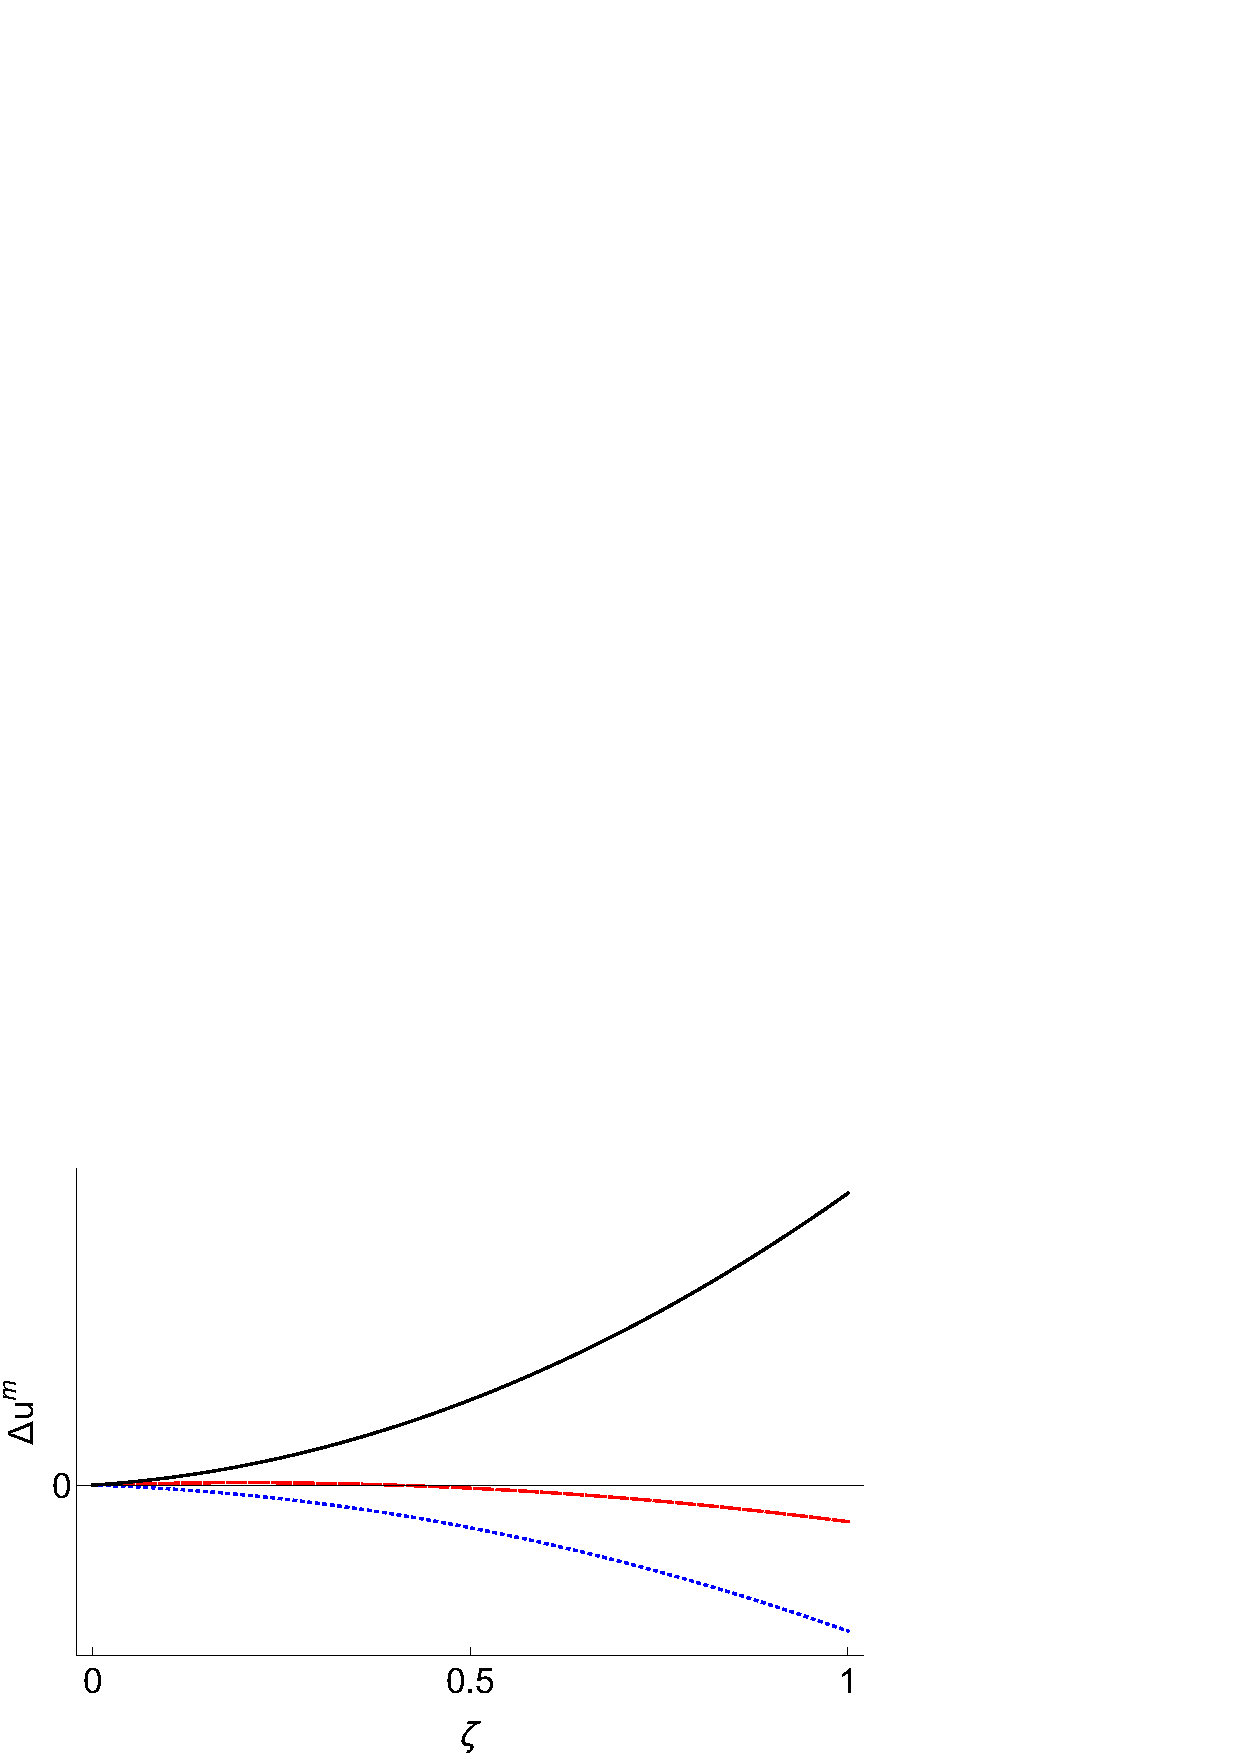
\includegraphics[width=\textwidth]{./Figures/Figure_Welfare_TgtSize.pdf}
      \end{subfigure}

      \bigskip


      \begin{subfigure}{.6\textwidth}
        \caption{{Utility gains of stabilization over strength of
            stabilization for stabilizing countries of different
            sizes}}
        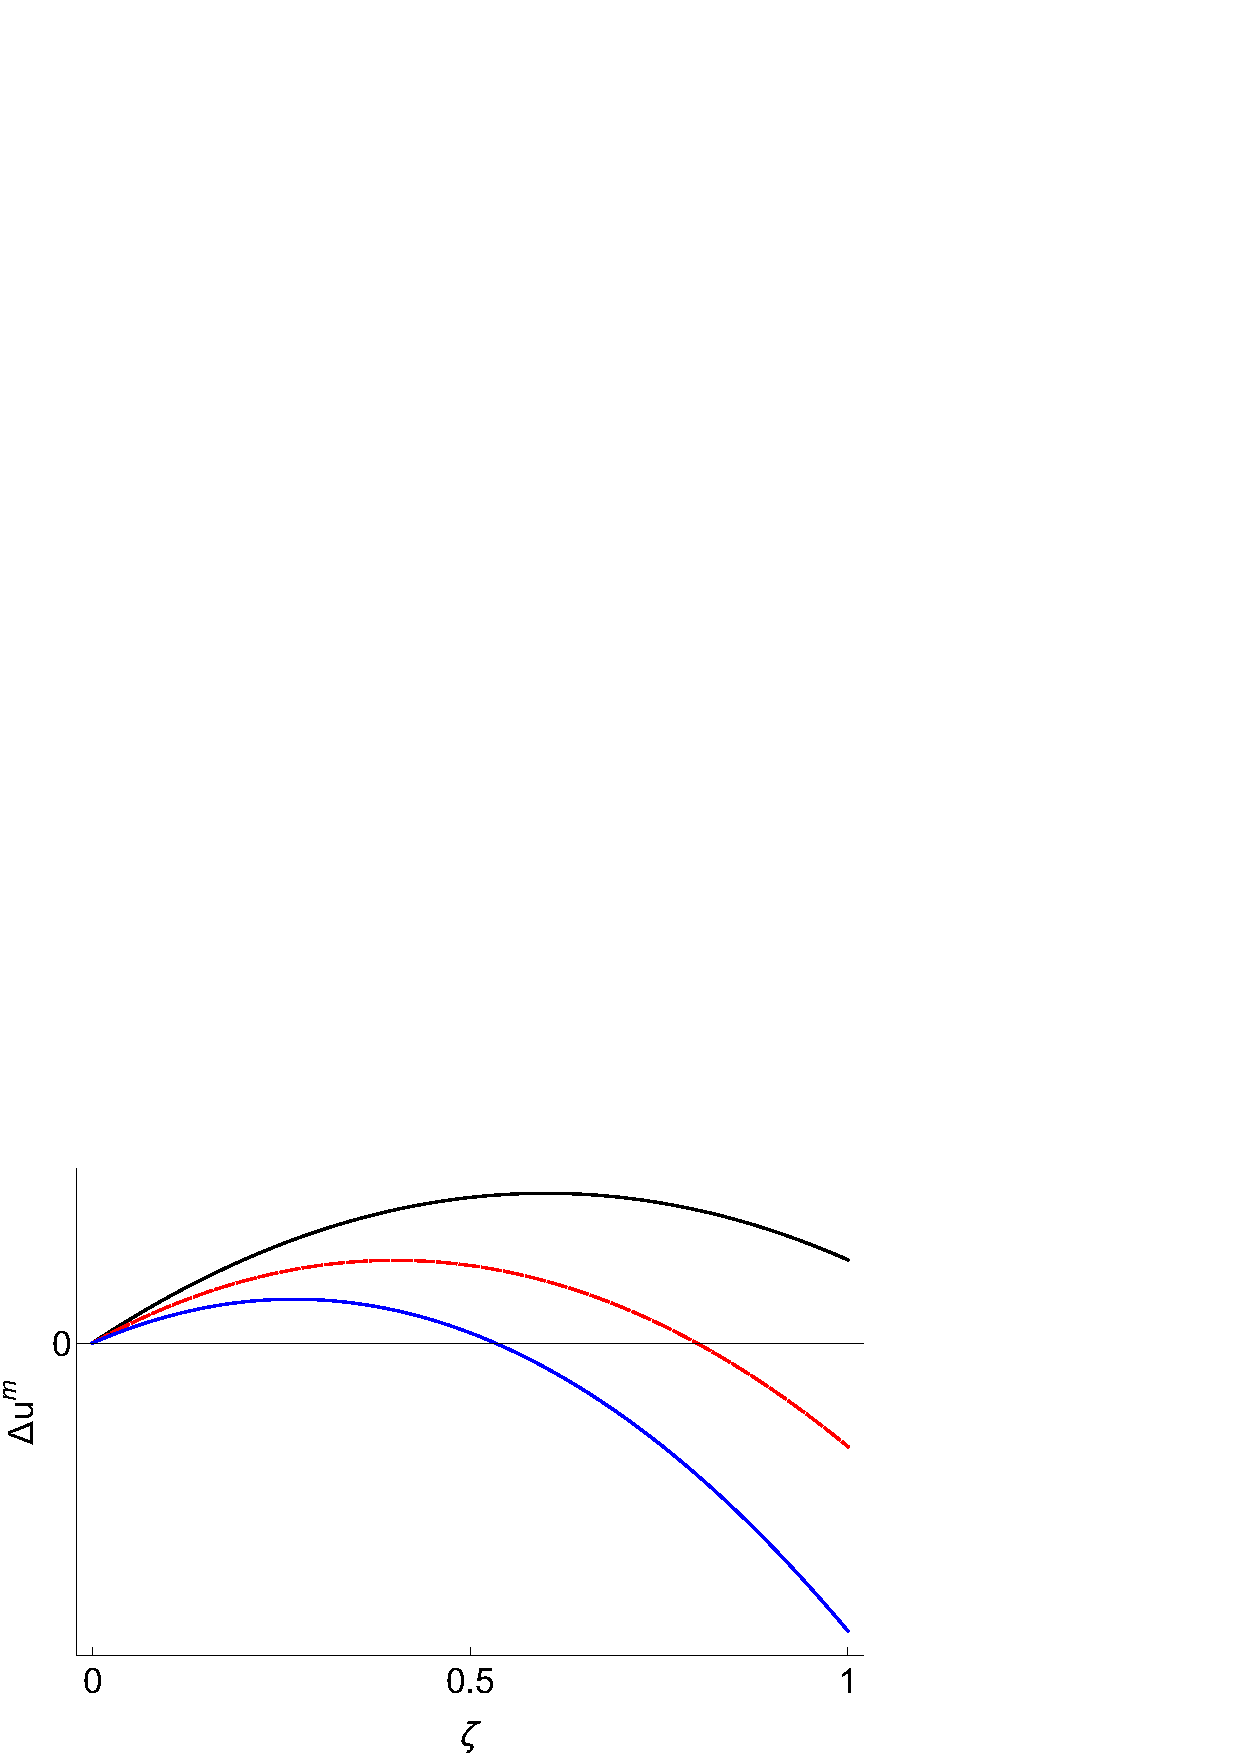
\includegraphics[width=\textwidth]{./Figures/Figure_Welfare_ThreeSizes.pdf}
      \end{subfigure}

\end{centering}
\bigskip

\small \textit{Notes:} Both plots show the percentage increase in the
certainty-equivalent consumption of a representative household in the
stabilizing country attributable to the stabilization ($\Delta u^m $)
for a numerical example where \(\tau=1/3\), and \(\gamma=7\). Panel
(a) shows the three components of $\Delta u^m $ shown on the right
hand side of (\ref{eq:Deltau}) for a small stabilizing country
($\theta^m=0$) and a hard peg (\(\zeta=1\)). The net utility gain is
the sum of the three lines. It is positive for all
\(\theta^t>\bar{\theta}\). Panel (b) shows the net utility gain as a
function of \(\zeta\) for stabilizing countries of different sizes.
See Appendix \ref{Appendix_Welfare} for the generalization of
(\ref{eq:Deltau}) that allows for $\theta^m>0$. \end{minipage}
\end{figure}

\clearpage

\begin{sidewaysfigure}[!h]
  \begin{minipage}{\linewidth}
    \begin{centering}
      \caption{Optimal Stabilizations}\label{fig_optimal}
      \begin{subfigure}{.49\textwidth}
        \caption{Optimal Choice of Exchange Rate Regime}
        \includegraphics[width=\textwidth]{./Figures/Figure_Optimal_Policy_1.jpg}
      \end{subfigure}
      \begin{subfigure}{.49\textwidth}
        \caption{Externalities on Target and Outside Countries}
        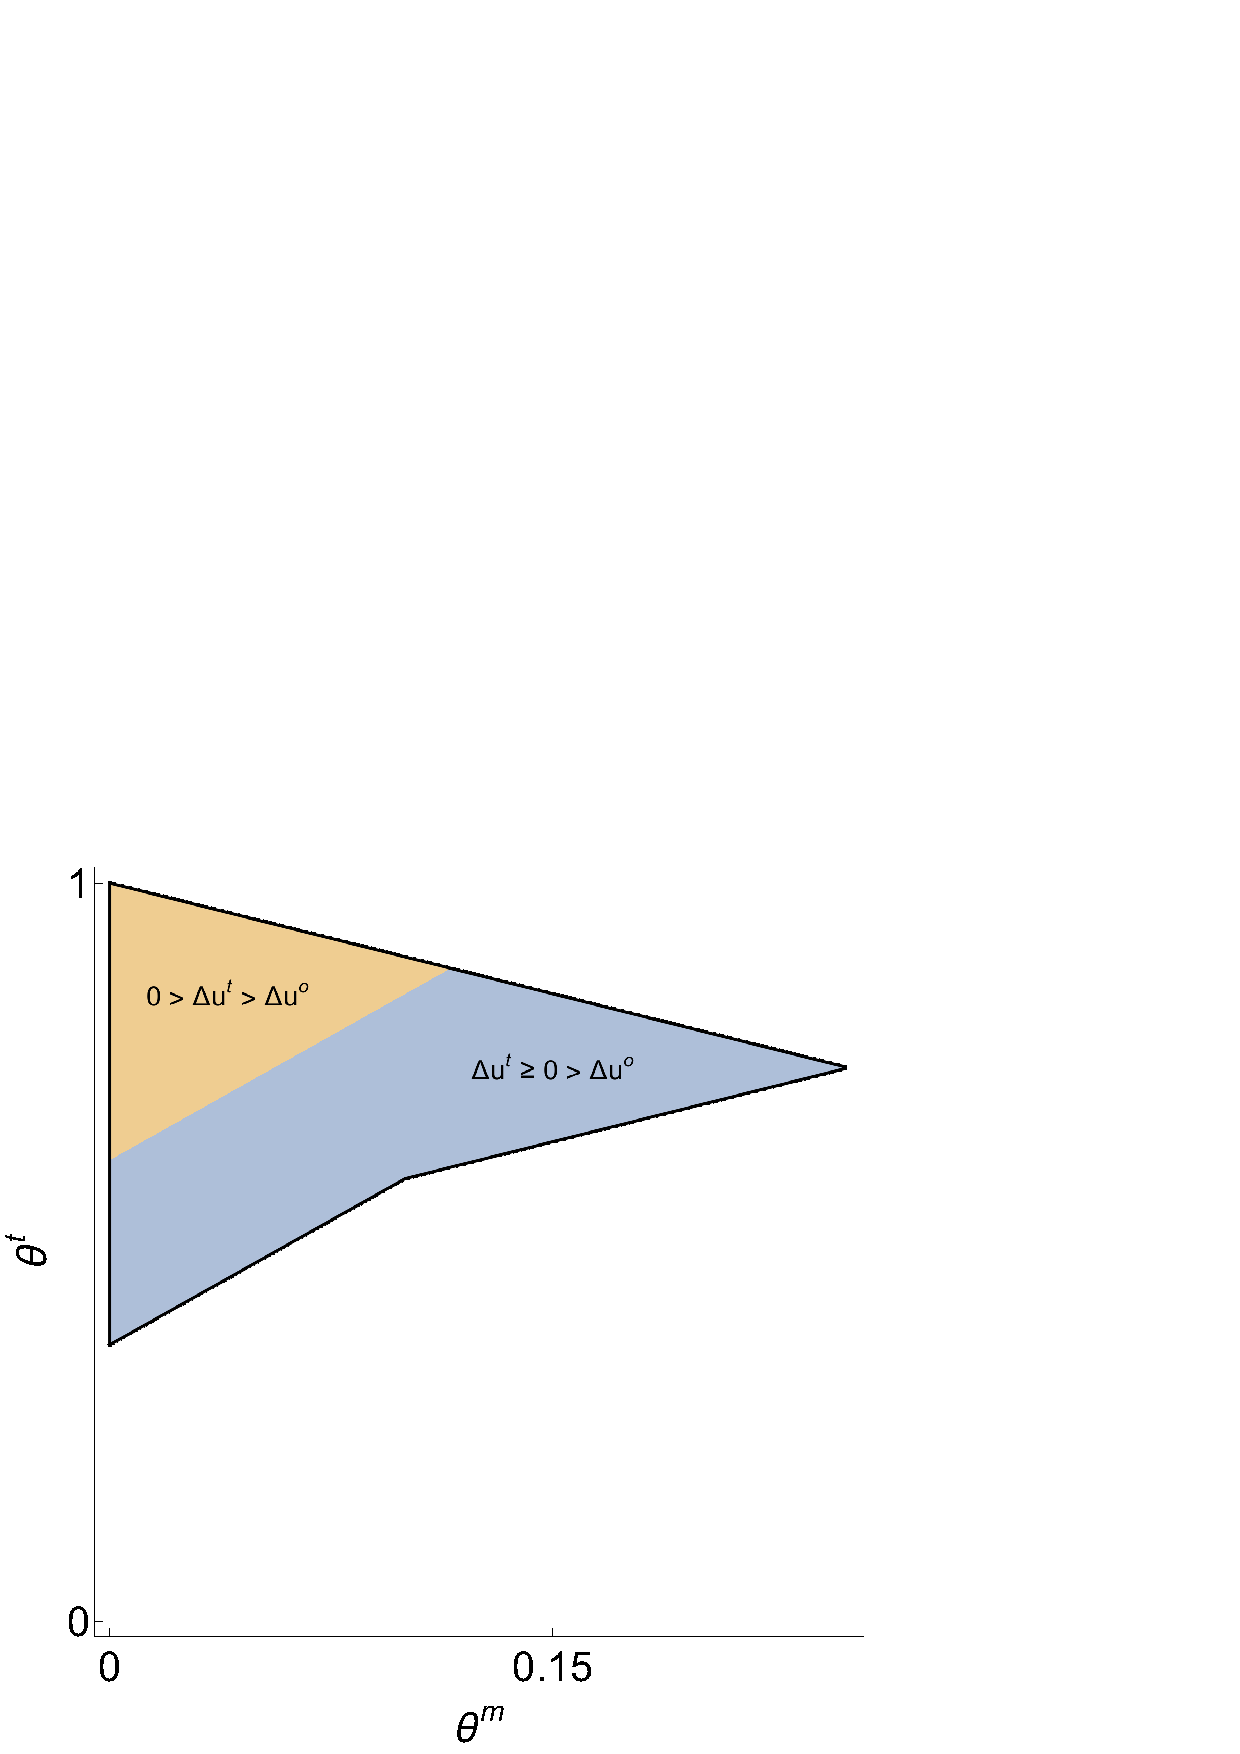
\includegraphics[width=\textwidth]{./Figures/Figure_Winners_and_Losers.pdf}
      \end{subfigure}

    \end{centering}

    \bigskip \small \textit{Notes:} The triangular region shown in
    both figures marks the subset of the parameter space where a
    stabilization is strictly welfare-increasing for the stabilizing
    country ($\Delta u^m>0 $) for a numerical example where
    \(\tau=1/3\), and \(\gamma=7\). Outside of triangular region the
    stabilizing country maximizes its own utility by floating
    ($\zeta=0 $). Panel (a) marks regions where the stabilizing
    country's optimal choice is to impose a hard peg ($\zeta=1 $,
    marked in red) versus a ``softer'' stabilization
    ($\zeta\in (0,1) $, marked in purple). Panel (b) illustrates the
    (pecuniary) externalities of these optimal stabilizations on the
    target and outside countries. \end{minipage}
\end{sidewaysfigure}

\clearpage
